%========================================================
% CHAPTER 4: RESULTS
%========================================================
\chapter{Results}
\label{chap:results}

This chapter reports four empirical findings, each building on the last. The through-line is a single claim: ESG change, not ESG level, is the operative pricing variable. The four sections establish this sequentially --- first ruling out a static cross-sectional greenium, then documenting contemporaneous and predictive effects of $\Delta$ESG, and finally revealing the Beta Amplification Paradox. 

%----------------------------------------------------
\section{Full Hypothesis Test Table}
%----------------------------------------------------
 
\begin{table}[H]
  \centering
  \caption{Complete Hypothesis Test Summary. Bonferroni threshold: $\alpha/6 \approx 0.008$. BH-FDR at $q=0.05$.}
  \label{tab:hyp_full}
  \small
  \begin{tabular}{lllccccc}
    \toprule
    ID & Research Q & Model & Coeff & Raw $p$ & Bonf.\ $p$ & BH $p$ & Decision \\
    \midrule
    H1 & ESG level within-FE     & M2  & 0.014  & 0.0002 & 0.0012 & 0.0083 & Reject*** \\
    H2 & ESG level cross-section & FM  & 0.0045 & 0.2797 & 1.000  & 0.050  & F.t.r. \\
    H3 & $\Delta$ESG contemp.    & M6  & 0.0203 & 0.0167 & 0.1002 & 0.0333 & Reject** \\
    H4 & ESG momentum (FF5)      & P3  & 0.0243 & 0.0017 & 0.0102 & 0.0167 & Reject*** \\
    H5 & $\Delta$ESG$\times$Mkt  & M6  & 0.5304 & 0.0049 & 0.0294 & 0.0250 & Reject*** \\
    H6 & ESG level$\times$Mkt    & M2C & 0.1063 & 0.1492 & 0.8952 & 0.0417 & F.t.r. \\
    \bottomrule
  \end{tabular}
  \smallskip\\
  \footnotesize F.t.r.\ $=$ Fail to reject. H3--H5 survive BH-FDR at $q=0.05$; H1 and H4 survive Bonferroni.
\end{table}

%----------------------------------------------------
\section{ESG Level: No Cross-Sectional Greenium (H1, H2)}
\label{sec:level}
%----------------------------------------------------

\subsection*{Within-Firm Level Effect (H1)}

Model M2 regresses excess returns on market risk and the time-varying ESG level with entity and year fixed effects. The within-FE coefficient is $\hat{\beta}_2 = 0.0140$ (SE $= 0.0038$, $t = 3.691$, $p = 0.0002$), surviving Bonferroni correction ($p_{\text{Bonf}} = 0.0012$). In months where a firm's normalised ESG score is 0.10 above its own historical average, excess return is approximately 14 basis points higher, conditional on market risk. This is a within-firm signal --- it says that firms become more valuable to investors when they are above their own ESG baseline, regardless of where that baseline sits in the cross-section.

\begin{figure}[H]
  \centering
  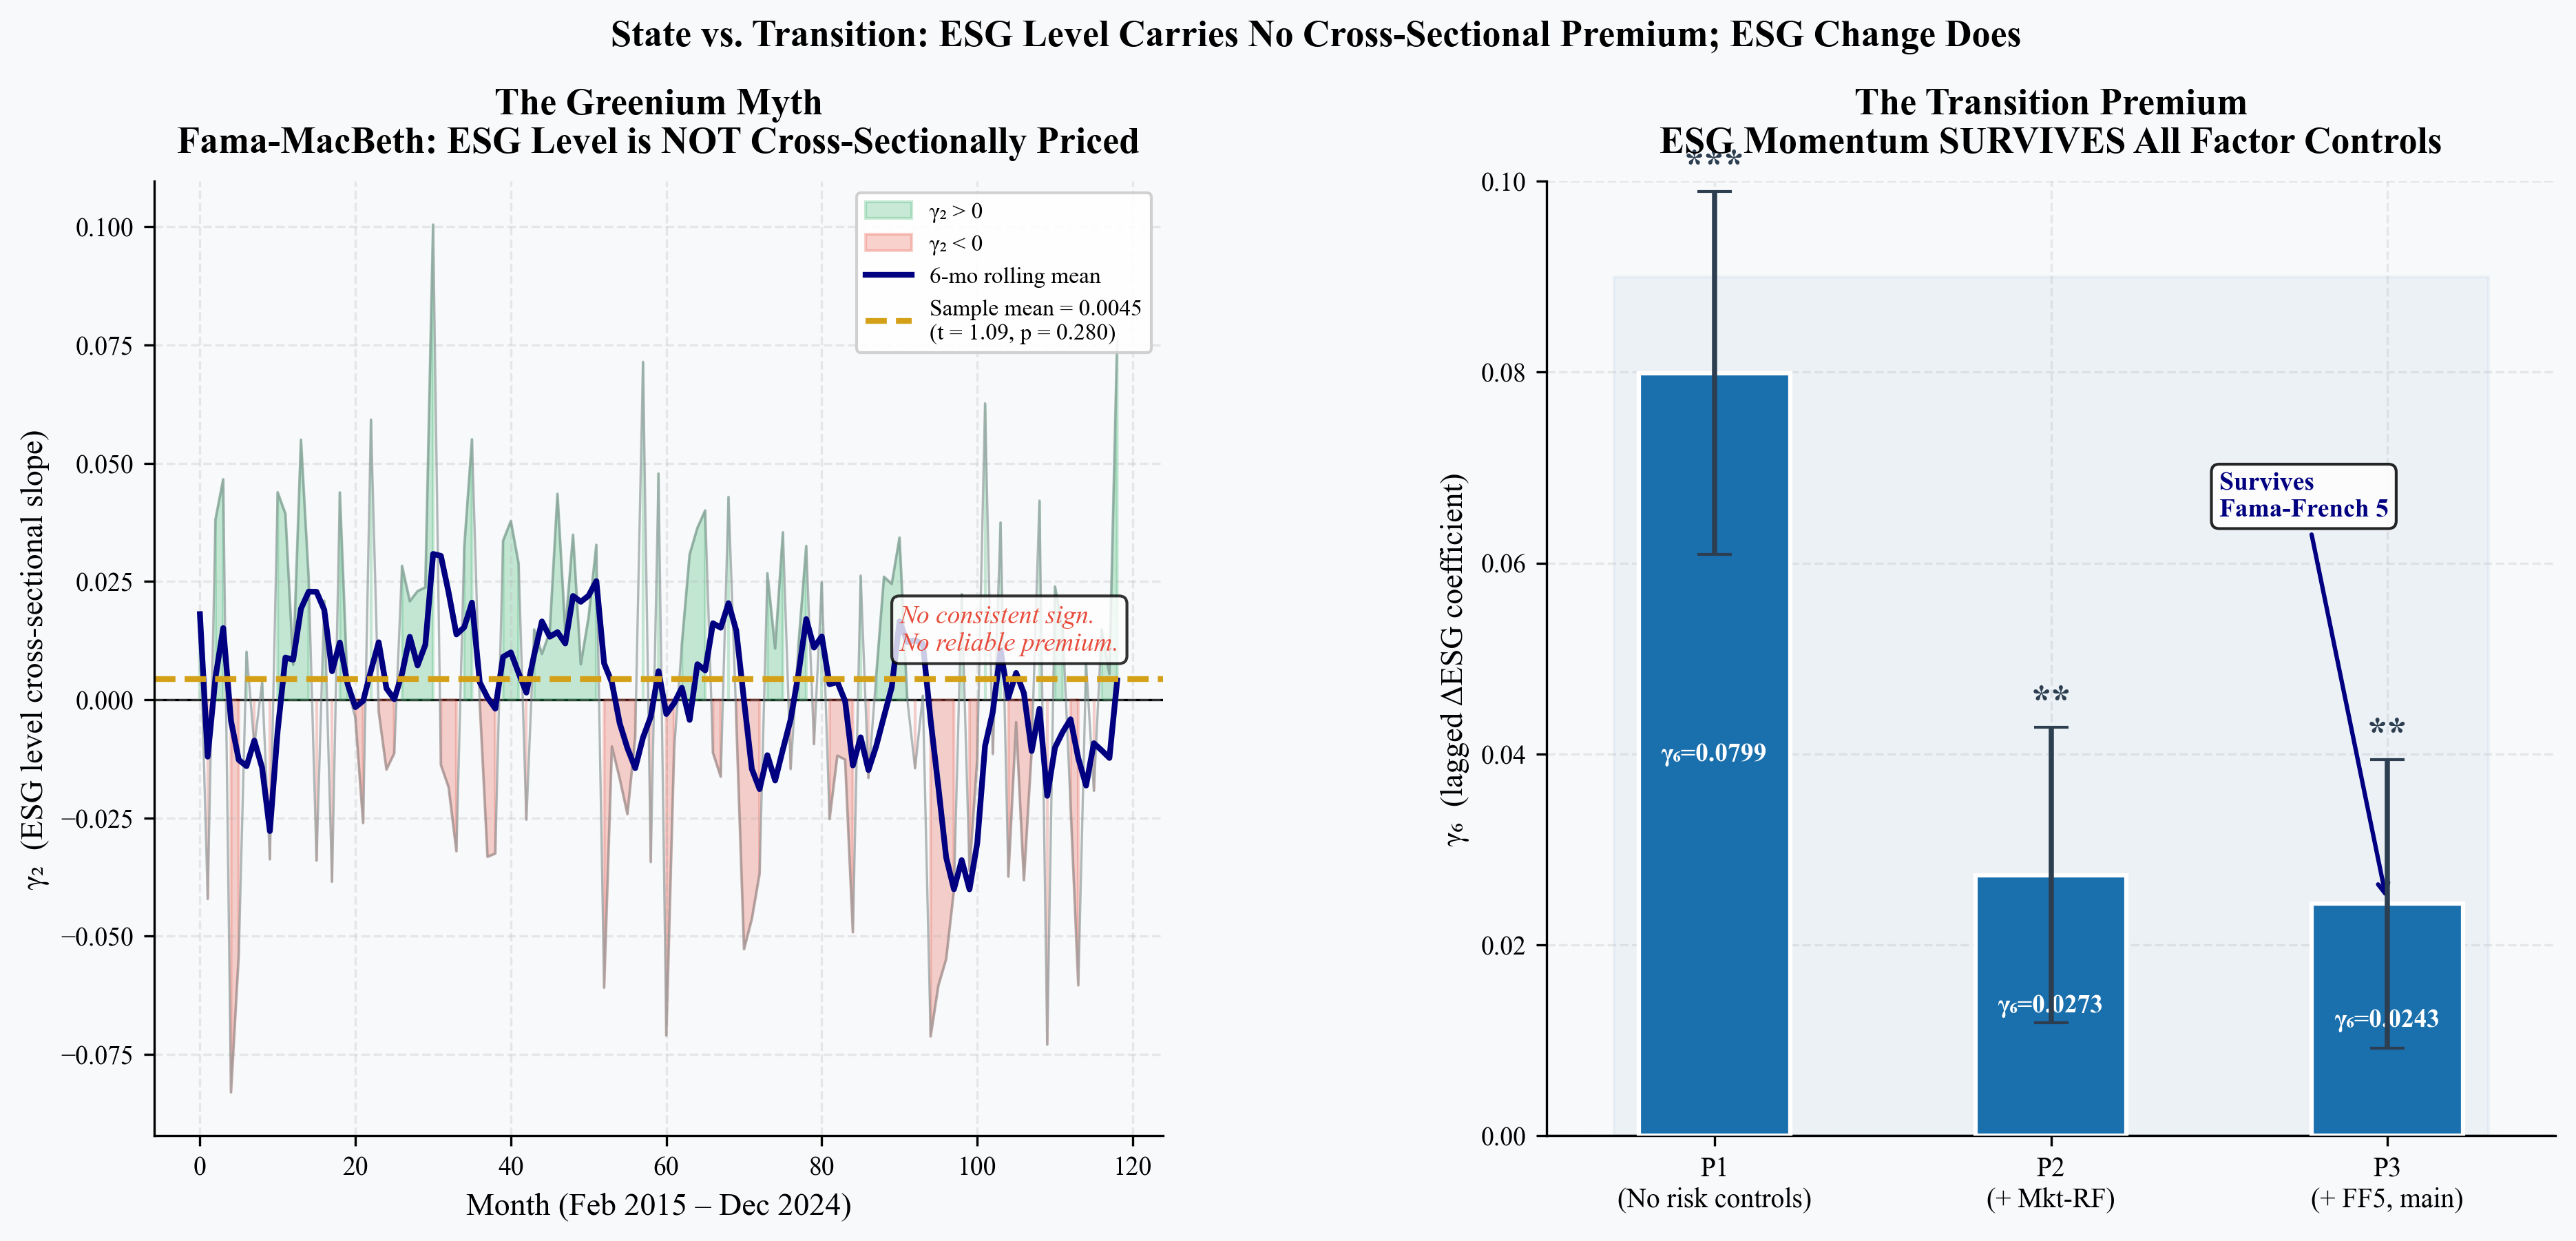
\includegraphics[width=\textwidth]{../Pictures/fig1_greenium_vs_transition.png}
  \caption{\textbf{Figure 5a --- Monthly ESG Coefficient (Fama-MacBeth) /  Monthly Cross-Sectional $R^2$.}
  Top: monthly cross-sectional ESG slope $\hat{\gamma}_{2,t}$; dashed line = full-sample mean. The irregular sign changes confirm that ESG level carries no persistent cross-sectional premium. Bottom: monthly $R^2$ across cross-sections.}
  \label{fig:fama_macbeth}
\end{figure}

\subsection*{No Cross-Sectional Premium (H2)}

The Fama-MacBeth test, however, tells a different story. Table~\ref{tab:fm} shows that the mean monthly ESG slope coefficient across 119 cross-sections is $\bar{\gamma}_2 = 0.00446$ with a Newey-West $t$-statistic of 1.086 ($p = 0.280$). ESG level does not command a reliable cross-sectional return premium. Figure~\ref{fig:fama_macbeth} confirms that the monthly ESG coefficient fluctuates in sign and magnitude throughout the sample, with no consistent direction.

\begin{table}[H]
  \centering
  \caption{Fama-MacBeth Cross-Sectional Regressions (H2). Mean slope coefficients with Newey-West standard errors (12 lags) across 119 monthly cross-sections. 479 firms.}
  \label{tab:fm}
  \begin{tabular}{lccccc}
    \toprule
    & $\bar{\gamma}$ & NW SE & $t$ & $p$ & Decision \\
    \midrule
    $\hat{\gamma}_0$ (intercept)   & 0.00110 & 0.00412 & 0.266 & 0.791 & --- \\
    $\hat{\gamma}_1$ (market beta) & 0.00864 & 0.00555 & 1.557 & 0.122 & F.t.r. \\
    $\hat{\gamma}_2$ (ESG level)   & 0.00446 & 0.00411 & 1.086 & \textbf{0.280} & F.t.r. \\
    \bottomrule
  \end{tabular}
  \smallskip\\
  \footnotesize F.t.r.\ $=$ Fail to reject. ESG$_{i,t}$ is time-varying normalised score; higher $=$ better ESG.
\end{table}



\noindent\textbf{Interpretation.} The divergence between H1 and H2 is itself a substantive finding. ESG level matters relative to a firm's own baseline (H1 rejects), but not as a cross-sectional characteristic separating high-ESG from low-ESG firms (H2 fails to reject). Static high ESG scores are already reflected in equilibrium prices. The return signal lives in the movement toward that score, not in the score itself.

%----------------------------------------------------
\section{ESG Changes Are Priced Contemporaneously (H3)}
\label{sec:change}
%----------------------------------------------------

\subsection*{The Aggregate Signal: Model M6}

Table~\ref{tab:panel} reports Models M1, M2, M2C, and M6 side by side. The key result is in M6: $\hat{\beta}_2 = 0.0203$ (SE $= 0.0085$, $t = 2.394$, $p = 0.017$). Within a given firm, a month in which the normalised ESG score improves by one unit above its mean is associated with a 2.03-percentage-point increase in excess return in that same month. This holds after conditioning on market risk, entity fixed effects, and year fixed effects. The economic mechanism is information flow: a rating revision signals changes in regulatory risk, governance quality, or operational sustainability that the market prices within the month. For large-cap S\&P 500 firms, rapid pricing is expected.

\subsection*{The Component-Level Failure: An Aggregate Synergy Signal}

When the composite $\Delta\mathrm{ESG}^c$ in M6 is replaced by the individual pillar changes $\Delta E^c$, $\Delta S^c$, and $\Delta G^c$ estimated separately, all three yield statistically insignificant coefficients: Environmental ($t = -0.201$, $p = 0.841$), Social ($t = 0.821$, $p = 0.411$), and Governance ($t$ not separately significant). The same pattern holds in the predictive specification (P3): $\Delta E^c$ ($t = -0.499$, $p = 0.618$), $\Delta S^c$ ($t = -0.565$, $p = 0.572$), $\Delta G^c$ ($t = -0.276$, $p = 0.782$) --- all insignificant.

This is a substantive finding. The market does not price changes to a firm's environmental footprint, its social practices, or its governance structure when considered in isolation. It prices the \emph{holistic composite}. Individual pillars carry too much idiosyncratic noise to move asset prices on their own; the Sustainalytics aggregate ESG score acts as a ``monolith'' rating that the market treats as a single, credible signal. This finding is consistent with the SASB materiality framework: what matters is the overall credibility of a firm's sustainability transition, not which specific dimension drives it.


\begin{table}[H]
  \centering
  \caption{Panel Fixed Effects Regressions (M1--M6). Dependent variable: monthly excess return. Entity and year FE. Standard errors clustered by firm.}
  \label{tab:panel}
  \begin{tabular}{lcccc}
    \toprule
    & M1 & M2 & M2C & M6 \\
    & CAPM & $+$ESG Level & $+$ESG$\times$Mkt & $+\Delta$ESG$\times$Mkt \\
    \midrule
    Mkt-RF                           & 0.9765*** & 0.9771*** & 0.9770*** & 0.9783*** \\
                                      & (0.0151)  & (0.0151)  & (0.0151)  & (0.0151)  \\[3pt]
    $\mathrm{ESG}_{i,t}$             &           & 0.0140*** &           &           \\
                                      &           & (0.0038)  &           &           \\[3pt]
    $\mathrm{ESG}_{i,t}^c$           &           &           & 0.0129*** &           \\
                                      &           &           & (0.0039)  &           \\[3pt]
    $\mathrm{ESG}_{i,t}^c\times$ Mkt-RF &        &           & 0.1063    &           \\
                                      &           &           & (0.0737)  &           \\[3pt]
    $\Delta\mathrm{ESG}_{i,t}^c$     &           &           &           & 0.0203**  \\
                                      &           &           &           & (0.0085)  \\[3pt]
    $\Delta\mathrm{ESG}_{i,t}^c\times$ Mkt-RF & &           &           & 0.5304*** \\
                                      &           &           &           & (0.1885)  \\[3pt]
    \midrule
    Entity FE                         & Yes & Yes & Yes & Yes \\
    Year FE                           & Yes & Yes & Yes & Yes \\
    $N$                               & 56,656 & 56,656 & 56,656 & 55,715 \\
    $R^2$                             & 0.2979 & 0.2980 & 0.2981 & 0.2991 \\
    Adj.\ $R^2$                       & 0.2917 & 0.2919 & 0.2920 & 0.2928 \\
    \bottomrule
  \end{tabular}
  \smallskip\\
  \footnotesize $^{***}p<0.01$, $^{**}p<0.05$, $^{*}p<0.10$. Superscript $c$ denotes mean-centred. M2C tests ESG-level beta modulation (H6: $t=1.442$, $p=0.149$, fails to reject). M6 tests $\Delta$ESG beta modulation (H5: $t=2.814$, $p=0.005$, rejects).
\end{table}


\noindent\textbf{Key message.} ESG improvements increase contemporaneous excess returns ($t=2.394$, $p=0.017$). Individual E, S, and G changes do not. The market prices the aggregate ESG change as an integrated information signal.

%----------------------------------------------------
\section[Lagged ESG Change Predicts Returns (H4)]{ESG Momentum: Lagged $\Delta$ESG Predicts Returns (H4)}
\label{sec:momentum}
%----------------------------------------------------

The predictive regressions P1--P3 test whether last month's ESG change forecasts this month's excess return. Table~\ref{tab:pred} shows results.

\begin{table}[H]
  \centering
  \caption{ESG Momentum: Predictive Regression Results (H4). Key variable: lagged $\Delta\mathrm{ESG}_{i,t-1}^c$. Entity and year FE. Firm-clustered SEs. $N=55{,}219$.}
  \label{tab:pred}
  \begin{tabular}{llccccc}
    \toprule
    Model & Controls & $\hat{\gamma}_6$ & SE & $t$ & $p$ & $R^2$ \\
    \midrule
    P1 & Entity + Year FE only & 0.0799 & 0.0097 & 8.251 & $<$0.001*** & 0.017 \\
    P2 & $+$ Mkt-RF            & 0.0273 & 0.0079 & 3.430 & 0.001***    & 0.301 \\
    P3 & $+$ FF5 (main)        & 0.0243 & 0.0077 & 3.140 & \textbf{0.002}*** & 0.306 \\
    \bottomrule
  \end{tabular}
  \smallskip\\
  \footnotesize $^{***}p<0.01$. P3 is the key specification: $\hat{\gamma}_6$ survives full Fama-French five-factor controls. The monotone attenuation from P1 to P3 confirms that part of the raw ESG predictability is absorbed by systematic risk factors, but a significant residual remains.
\end{table}

In P3, $\hat{\gamma}_6 = 0.0243$ ($t = 3.14$, $p = 0.002$), significant at the 1\% level and surviving Bonferroni correction ($p_{\text{Bonf}} = 0.010$). A firm that improved its ESG profile last month will --- all else equal --- earn higher excess returns this month even after market, size, value, profitability, and investment factors are controlled. Figure~\ref{fig:momentum} illustrates the economic magnitude: firms in the top quintile of lagged ESG improvement earn substantially higher next-month returns than those in the bottom quintile, with a near-monotone gradient.

\begin{figure}[H]
  \centering
  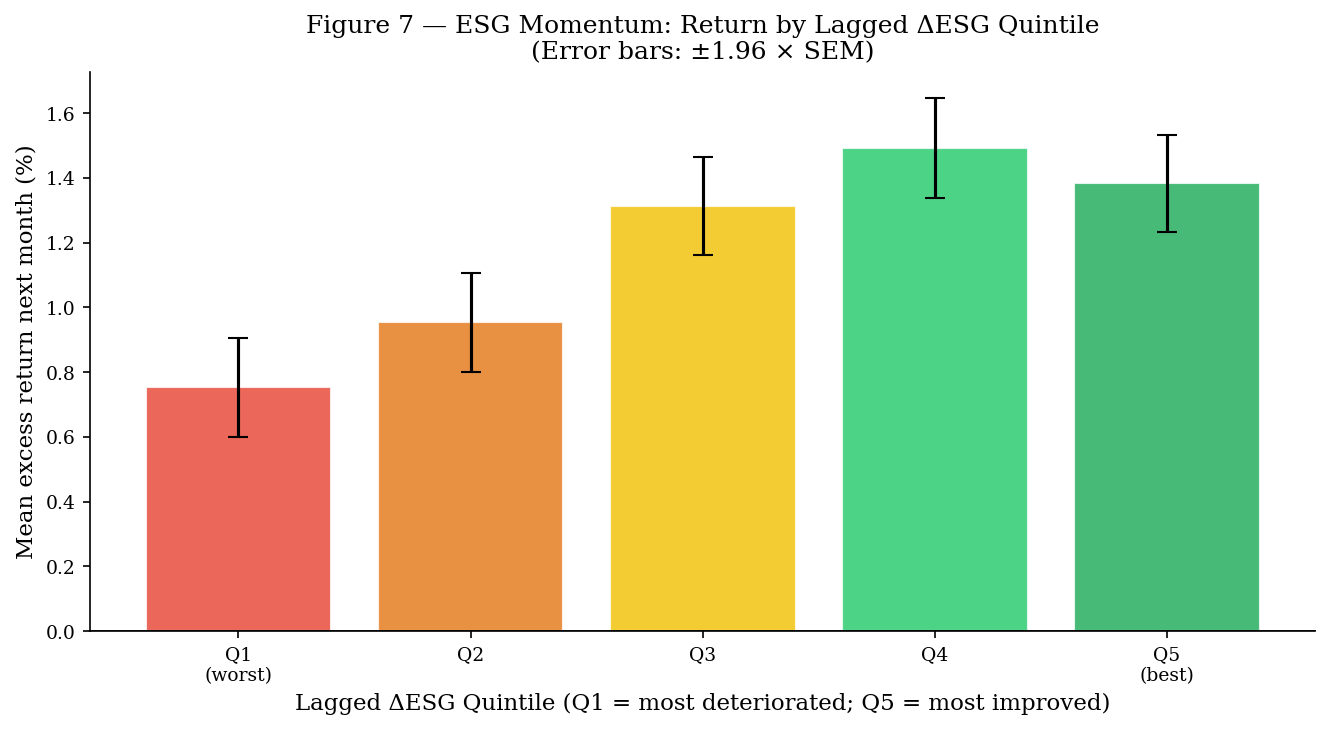
\includegraphics[width=0.82\textwidth]{../Pictures/fig7_esg_momentum.png}
  \caption{\textbf{Figure 5c --- ESG Momentum: Return by Lagged ESG Change Quintile.}
  Mean monthly excess return in the following period for firms sorted by quintile of lagged $\Delta\mathrm{ESG}_{i,t-1}^c$. Q1 = most deteriorated; Q5 = most improved. Error bars: $\pm1.96\times\mathrm{SEM}$. The monotone pattern confirms the ESG momentum channel documented in P1--P3.}
  \label{fig:momentum}
\end{figure}

The mechanism is gradual institutional rebalancing. ESG-screened mandates respond to score changes by adjusting holdings over multiple months due to position size constraints and mandate-driven rebalancing cycles. This creates a persistent demand shock that extends the price impact of an ESG improvement beyond the contemporaneous month, generating the predictability documented in P3.

\noindent\textbf{Key message.} ESG changes predict future returns ($t=3.14$, $p=0.002$). The market does not immediately and fully price ESG information: there is a momentum channel that generates exploitable next-month predictability net of five systematic risk factors.

%----------------------------------------------------
\section{The Beta Amplification Paradox (H5, H6)}
\label{sec:beta}
%----------------------------------------------------

\subsection*{$\Delta$ESG Amplifies Market Beta --- Not ESG Level}

The most original finding of this thesis concerns the interaction between ESG change and market risk. Returning to Table~\ref{tab:panel}, the interaction term in M6 is $\hat{\beta}_3 = 0.5304$ (SE $= 0.1885$, $t = 2.814$, $p = 0.005$). ESG improvements significantly \emph{amplify} market beta. A one-unit increase in $\Delta\mathrm{ESG}^c$ raises the firm's effective market beta loading by 0.5304 --- a substantial economic magnitude. This stands in sharp contrast to M2C, where the ESG-\emph{level}-by-market interaction is statistically insignificant ($t = 1.442$, $p = 0.149$, H6 fails to reject). It is the dynamic of ESG change, not the static level, that modulates systematic risk.

The direction is paradoxical relative to conventional expectations. The standard narrative holds that better-managed, more sustainable firms are less sensitive to macroeconomic shocks, and therefore carry lower betas. Our evidence shows the opposite: firms actively improving their ESG profile temporarily \emph{increase} their market co-movement. We term this the Beta Amplification Paradox and offer two complementary explanations.

\textbf{Transition risk.} Firms improving ESG are in operational transition --- investing in new sustainability infrastructure, restructuring supply chains, and absorbing governance changes. These activities are capital-intensive and operationally disruptive, increasing the firm's sensitivity to the macroeconomic environment during the transition period. A recession during an ESG transition amplifies losses; an expansion amplifies gains.

\textbf{Correlated institutional flows.} ESG improvements attract correlated inflows from ESG-screened institutional mandates. As multiple ESG funds simultaneously accumulate shares in an improving firm, the firm's return becomes more tightly coupled to the aggregate market through the common factor in institutional demand. This artificially increases beta during the inflow phase.



\subsection*{Sector Materiality: Where the ESG Signal Is Priced}

Table~\ref{tab:sector} and Figure~\ref{fig:forest} disaggregate the $\Delta$ESG contemporaneous return effect by GICS sector. The result confirms the SASB materiality hypothesis: the ESG change signal is priced where it is financially material and ignored where it is not.
In capital-intensive sectors --- Materials, Industrials, Consumer Discretionary, Financials --- an ESG improvement represents a genuine operational overhaul: a chemical plant reducing emissions, a manufacturer improving supply-chain governance, a bank restructuring lending criteria for ESG risk. These are material changes that directly alter regulatory exposure and enterprise risk, and the market prices them accordingly. In Information Technology ($p = 0.670$), by contrast, ESG improvements are frequently viewed as immaterial CSR activity with no bearing on the firm's fundamental value drivers, and the market does not price them.

\begin{table}[H]
  \centering
  \caption{$\Delta$ESG Return Effect by GICS Sector. Entity and year FE within-sector regressions. Key variable: $\Delta\mathrm{ESG}_{i,t}^c$.}
  \label{tab:sector}
  \begin{tabular}{lccccc}
    \toprule
    Sector & $N$ firms & $\hat{\beta}_{\Delta\mathrm{ESG}}$ & SE & $t$ & $p$ \\
    \midrule
    Materials              & 24 & 0.1153 & 0.0409 & 2.82 & 0.005*** \\
    Consumer Discretionary & 46 & 0.0719 & 0.0272 & 2.65 & 0.008*** \\
    Industrials            & 74 & 0.0577 & 0.0213 & 2.71 & 0.007*** \\
    Financials             & 74 & 0.0467 & 0.0160 & 2.91 & 0.004*** \\
    \midrule
    Energy                 & 21 & 0.0326 & 0.0370 & 0.88 & 0.379  \\
    Communication Services & 21 & 0.0229 & 0.0380 & 0.60 & 0.546  \\
    Information Technology & 67 & 0.0108 & 0.0254 & 0.43 & \textbf{0.670}  \\
    Real Estate            & 31 & 0.0078 & 0.0237 & 0.33 & 0.743  \\
    Health Care            & 56 & $-$0.0023 & 0.0274 & $-$0.08 & 0.934 \\
    Utilities              & 30 & $-$0.0140 & 0.0181 & $-$0.77 & 0.440 \\
    Consumer Staples       & 35 & $-$0.0453 & 0.0239 & $-$1.90 & 0.057* \\
    \bottomrule
  \end{tabular}
  \smallskip\\
  \footnotesize $^{***}p<0.01$, $^{**}p<0.05$, $^{*}p<0.10$. Top four sectors significant; bottom seven not significant at 5\%.
\end{table}

\subsection{ESG Momentum and Market Stress: A Regime-Dependent Perspective}

To further investigate the conditions under which ESG momentum is priced, we examine the relationship between ESG momentum and market stress over time. Specifically, we compute the 12-month rolling correlation between the ESG momentum spread (Q5–Q1 portfolio returns) and a proxy for market stress, measured using market volatility.

Figure \ref{fig:esg_stress_corr} presents the time-varying correlation alongside the corresponding evolution of market volatility and the ESG momentum spread. The correlation exhibits substantial temporal variation, ranging from strongly negative values (approximately $-0.6$) in the early sample period to strongly positive values (above $0.6$) in later years.

\begin{figure}[H]
    \centering
    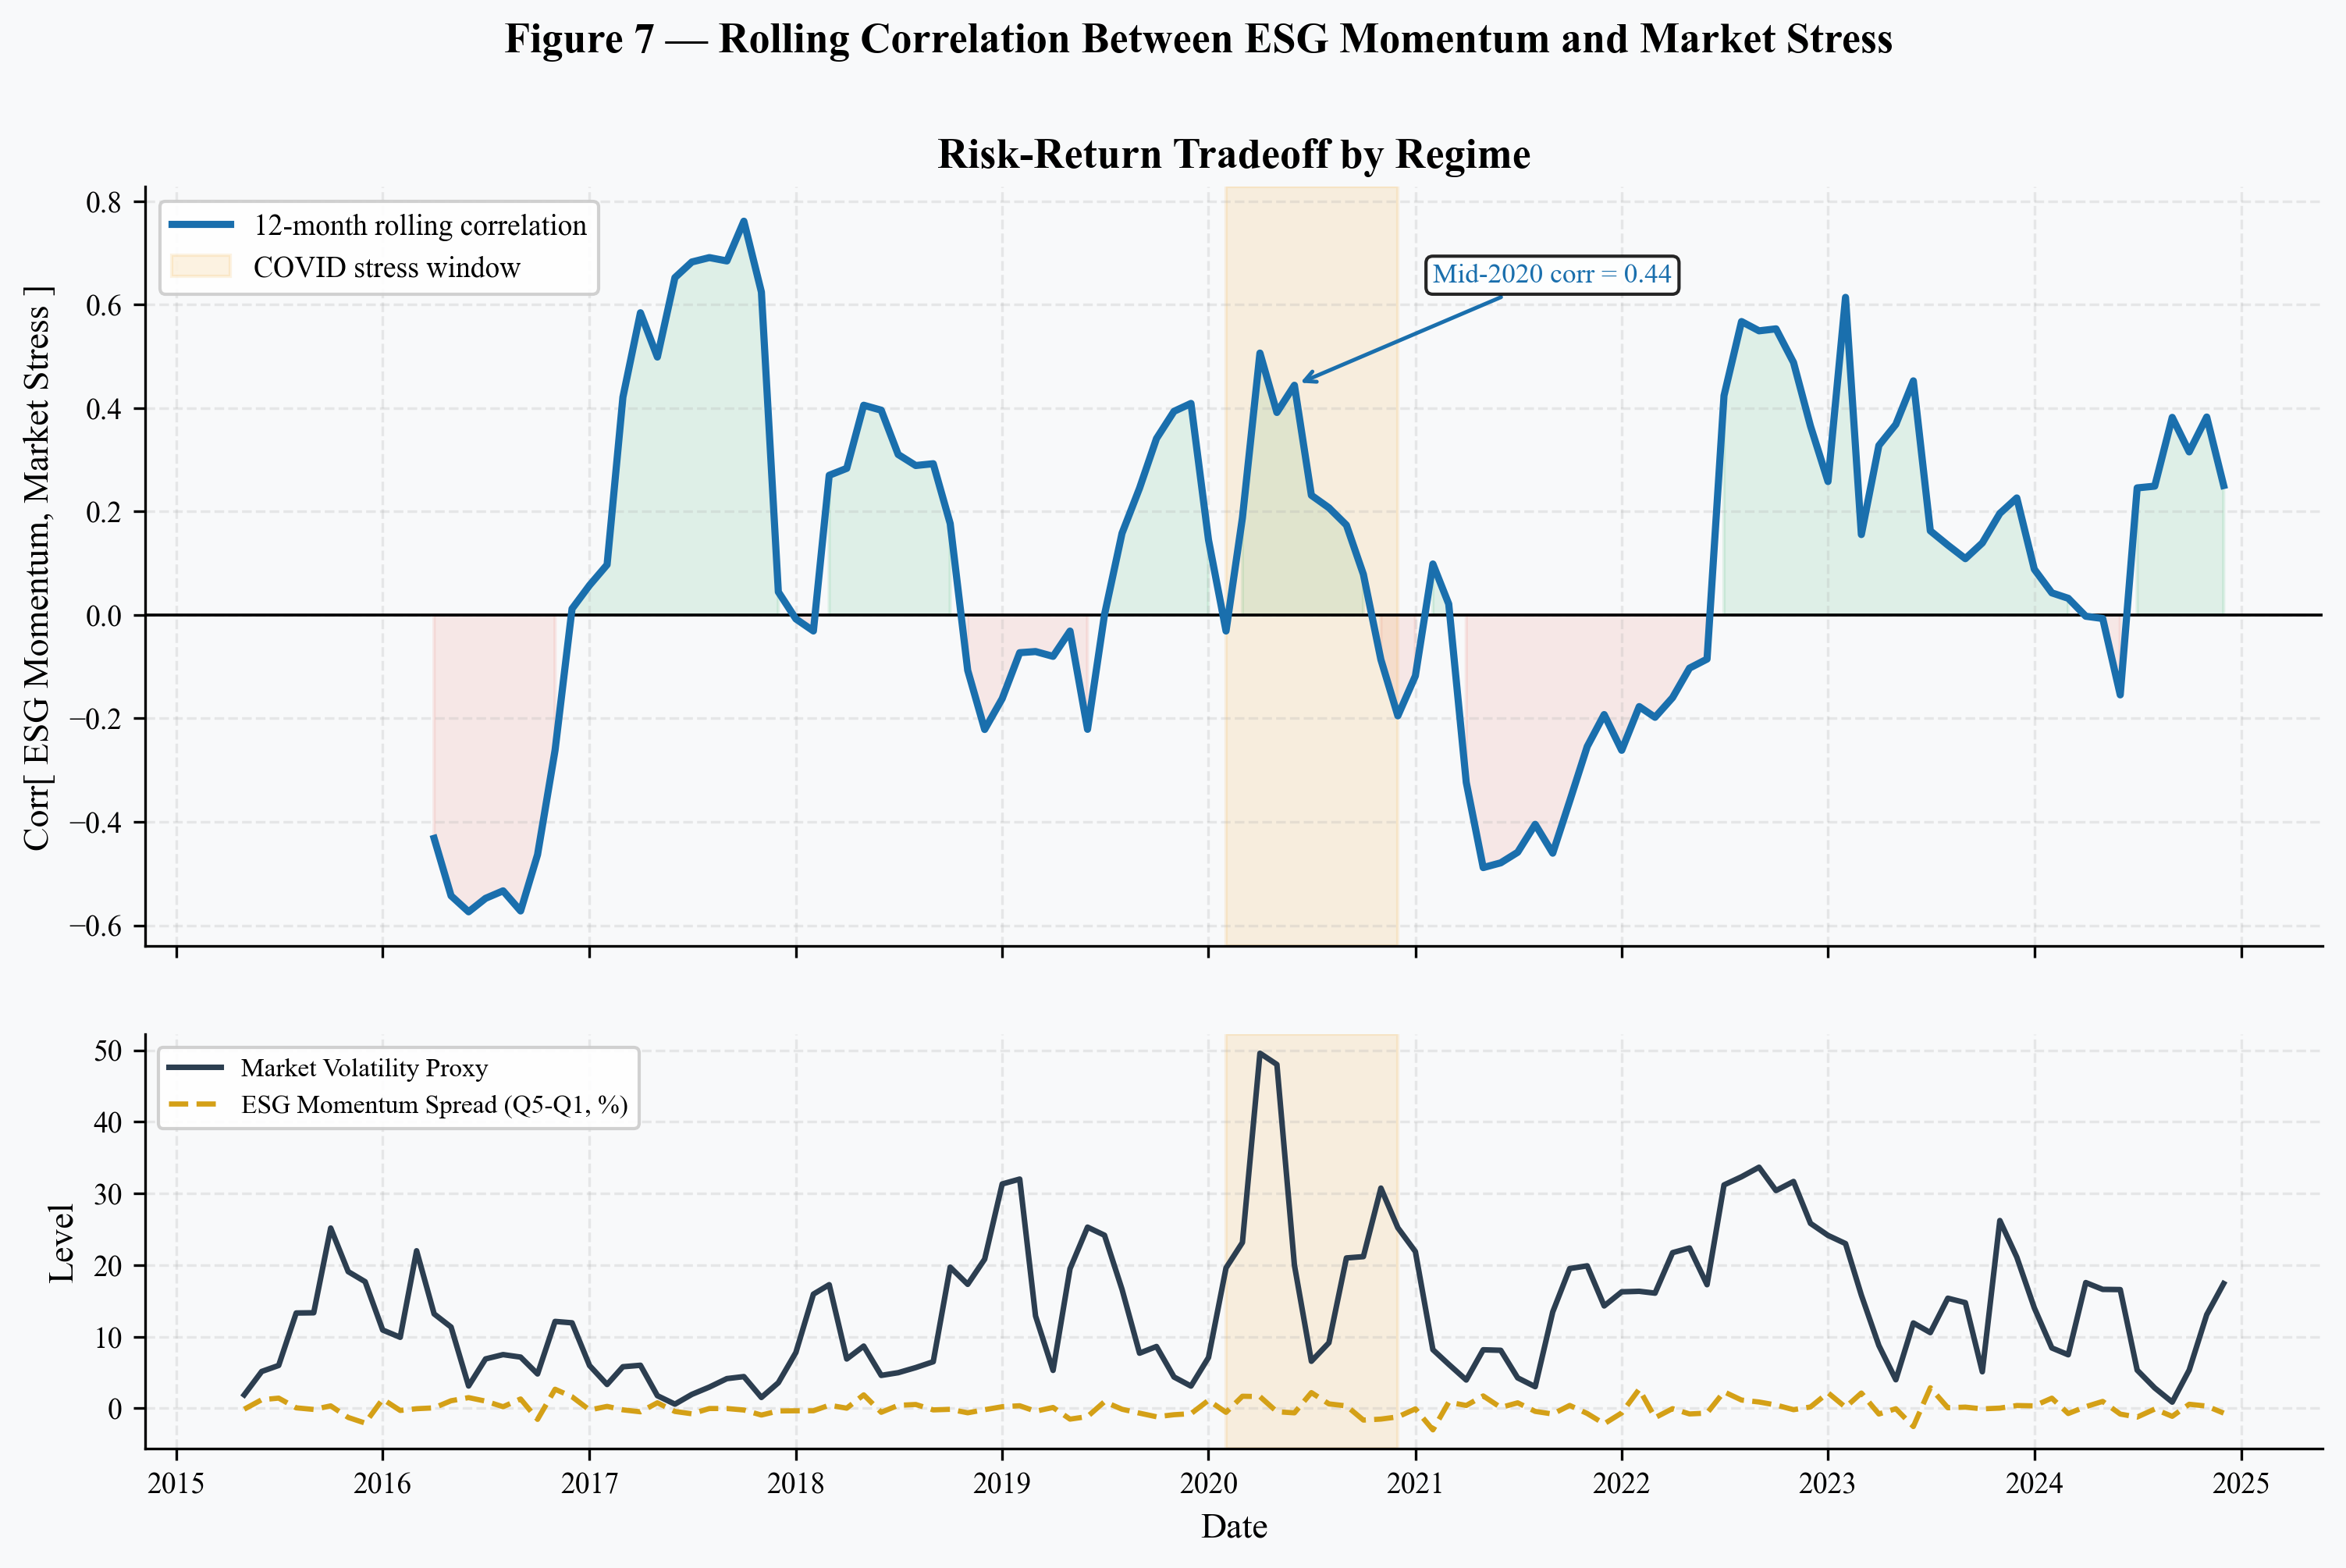
\includegraphics[width=0.9\linewidth]{../Pictures/fig7_regime_rolling_corr.png}
    \caption{Rolling Correlation Between ESG Momentum and Market Stress. 
    The top panel shows the 12-month rolling correlation between ESG momentum (Q5–Q1 spread) and a market volatility proxy. 
    The shaded region highlights the COVID-19 stress period (Jan 2020–Jun 2021). 
    The bottom panel displays the level of market volatility alongside the ESG momentum spread.}
    \label{fig:esg_stress_corr}
\end{figure}

A key observation emerges during the COVID-19 stress window. As market volatility spikes sharply, the rolling correlation turns significantly positive, reaching approximately $0.44$ at its peak. This indicates that ESG momentum strategies perform relatively better during periods of elevated market stress. In contrast, during calmer market conditions, the correlation weakens or turns negative, suggesting that ESG momentum is less consistently rewarded in low-volatility environments.

This evidence points to a regime-dependent structure in ESG pricing. ESG momentum does not behave as a static return factor; rather, its effectiveness depends critically on the prevailing market environment. During periods of heightened uncertainty, ESG improvements appear to act as a resilience signal, attracting capital flows toward firms perceived as more robust, better governed, or less exposed to downside risks.

The result complements the earlier findings on ESG momentum (H4) and the Beta Amplification Paradox (H5). While lagged ESG improvements generate statistically significant return predictability, the strength of this effect is conditional on market stress regimes. Taken together, the evidence suggests that ESG is best understood as a dynamic and state-dependent pricing factor, rather than a persistent cross-sectional premium.

